\documentclass{article}
\usepackage{graphicx, tikz-cd, float, titlepic, booktabs} % Required for inserting images
\usepackage{pgfplots}
\pgfplotsset{compat=1.15}
\usepackage{mathrsfs}
\usetikzlibrary{arrows}
\usepackage{amsmath, amssymb, amsthm, amsfonts, siunitx, physics, gensymb}
\AtBeginDocument{\RenewCommandCopy\qty\SI}
\usepackage[version=4]{mhchem}
\usepackage[most,many,breakable]{tcolorbox}
\usepackage{xcolor, fancyhdr, varwidth}
\usepackage[Glenn]{fncychap}
%Options: Sonny, Lenny, Glenn, Conny, Rejne, Bjarne, Bjornstrup
\usepackage{hyperref, cleveref}
\usepackage{icomma, enumitem} %comma as decimal and continue enumerate with [resume]
\usepackage{plimsoll}
\usepackage[danish]{babel}
%%%%%%%%%%%%%%%%%%%%%%%%%%%%%%
% SELF MADE COLORS
%%%%%%%%%%%%%%%%%%%%%%%%%%%%%%
\definecolor{myg}{RGB}{56, 140, 70}
\definecolor{myb}{RGB}{45, 111, 177}
\definecolor{myr}{RGB}{199, 68, 64}
\definecolor{mytheorembg}{HTML}{F2F2F9}
\definecolor{mytheoremfr}{HTML}{00007B}
\definecolor{mylenmabg}{HTML}{FFFAF8}
\definecolor{mylenmafr}{HTML}{983b0f}
\definecolor{mypropbg}{HTML}{f2fbfc}
\definecolor{mypropfr}{HTML}{191971}
\definecolor{myexamplebg}{HTML}{F2FBF8}
\definecolor{myexamplefr}{HTML}{88D6D1}
\definecolor{myexampleti}{HTML}{2A7F7F}
\definecolor{mydefinitbg}{HTML}{E5E5FF}
\definecolor{mydefinitfr}{HTML}{3F3FA3}
\definecolor{notesgreen}{RGB}{0,162,0}
\definecolor{myp}{RGB}{197, 92, 212}
\definecolor{mygr}{HTML}{2C3338}
\definecolor{myred}{RGB}{127,0,0}
\definecolor{myyellow}{RGB}{169,121,69}
\definecolor{myexercisebg}{HTML}{F2FBF8}
\definecolor{myexercisefg}{HTML}{88D6D1}
%%%%%%%%%%%%%%%%%%%%%%%%%%%%%%%%%%%%%%%%%%%%%%%%%%%%%%%%%%%%%%%%%%%%%%
% Box environments for theorems and problems
%%%%%%%%%%%%%%%%%%%%%%%%%%%%%%%%%%%%%%%%%%%%%%%%%%%%%%%%%%%%%%%%%%%%%
\setlength{\parindent}{1cm}
%================================
% Question BOX
%================================
\makeatletter
\newtcbtheorem{question}{Opgave}{enhanced,
	breakable,
	colback=white,
	colframe=myb!80!black,
	attach boxed title to top left={yshift*=-\tcboxedtitleheight},
	fonttitle=\bfseries,
	title={#2},
	boxed title size=title,
	boxed title style={%
			sharp corners,
			rounded corners=northwest,
			colback=tcbcolframe,
			boxrule=0pt,
		},
	underlay boxed title={%
			\path[fill=tcbcolframe] (title.south west)--(title.south east)
			to[out=0, in=180] ([xshift=5mm]title.east)--
			(title.center-|frame.east)
			[rounded corners=\kvtcb@arc] |-
			(frame.north) -| cycle;
		},
	#1
}{def}
\makeatother
%================================
% DEFINITION BOX
%================================

\newtcbtheorem[]{Definition}{Definition}{enhanced,
	before skip=2mm,after skip=2mm, colback=red!5,colframe=red!80!black,boxrule=0.5mm,
	attach boxed title to top left={xshift=1cm,yshift*=1mm-\tcboxedtitleheight}, varwidth boxed title*=-3cm,
	boxed title style={frame code={
					\path[fill=tcbcolback]
					([yshift=-1mm,xshift=-1mm]frame.north west)
					arc[start angle=0,end angle=180,radius=1mm]
					([yshift=-1mm,xshift=1mm]frame.north east)
					arc[start angle=180,end angle=0,radius=1mm];
					\path[left color=tcbcolback!60!black,right color=tcbcolback!60!black,
						middle color=tcbcolback!80!black]
					([xshift=-2mm]frame.north west) -- ([xshift=2mm]frame.north east)
					[rounded corners=1mm]-- ([xshift=1mm,yshift=-1mm]frame.north east)
					-- (frame.south east) -- (frame.south west)
					-- ([xshift=-1mm,yshift=-1mm]frame.north west)
					[sharp corners]-- cycle;
				},interior engine=empty,
		},
	fonttitle=\bfseries,
	title={#2},#1}{def}
\newtcbtheorem[]{definition}{Definition}{enhanced,
	before skip=2mm,after skip=2mm, colback=red!5,colframe=red!80!black,boxrule=0.5mm,
	attach boxed title to top left={xshift=1cm,yshift*=1mm-\tcboxedtitleheight}, varwidth boxed title*=-3cm,
	boxed title style={frame code={
					\path[fill=tcbcolback]
					([yshift=-1mm,xshift=-1mm]frame.north west)
					arc[start angle=0,end angle=180,radius=1mm]
					([yshift=-1mm,xshift=1mm]frame.north east)
					arc[start angle=180,end angle=0,radius=1mm];
					\path[left color=tcbcolback!60!black,right color=tcbcolback!60!black,
						middle color=tcbcolback!80!black]
					([xshift=-2mm]frame.north west) -- ([xshift=2mm]frame.north east)
					[rounded corners=1mm]-- ([xshift=1mm,yshift=-1mm]frame.north east)
					-- (frame.south east) -- (frame.south west)
					-- ([xshift=-1mm,yshift=-1mm]frame.north west)
					[sharp corners]-- cycle;
				},interior engine=empty,
		},
	fonttitle=\bfseries,
	title={#2},#1}{def}

\newtcbtheorem{theo}%
    {Theorem}{}{theorem}
\newtcolorbox{prob}[1]{colback=red!5!white,colframe=red!50!black,fonttitle=\bfseries,title={#1}}
%================================
% NOTE BOX
%================================

\usetikzlibrary{arrows,calc,shadows.blur}
\tcbuselibrary{skins}
\newtcolorbox{note}[1][]{%
	enhanced jigsaw,
	colback=gray!20!white,%
	colframe=gray!80!black,
	size=small,
	boxrule=1pt,
	title=\textbf{Note:},
	halign title=flush center,
	coltitle=black,
	breakable,
	drop shadow=black!50!white,
	attach boxed title to top left={xshift=1cm,yshift=-\tcboxedtitleheight/2,yshifttext=-\tcboxedtitleheight/2},
	minipage boxed title=1.5cm,
	boxed title style={%
			colback=white,
			size=fbox,
			boxrule=1pt,
			boxsep=2pt,
			underlay={%
					\coordinate (dotA) at ($(interior.west) + (-0.5pt,0)$);
					\coordinate (dotB) at ($(interior.east) + (0.5pt,0)$);
					\begin{scope}
						\clip (interior.north west) rectangle ([xshift=3ex]interior.east);
						\filldraw [white, blur shadow={shadow opacity=60, shadow yshift=-.75ex}, rounded corners=2pt] (interior.north west) rectangle (interior.south east);
					\end{scope}
					\begin{scope}[gray!80!black]
						\fill (dotA) circle (2pt);
						\fill (dotB) circle (2pt);
					\end{scope}
				},
		},
	#1,
}
%================================
% EXAMPLE BOX
%================================
\newtcbtheorem[number within=section]{Example}{Example}
{%
	colback = myexamplebg
	,breakable
	,colframe = myexamplefr
	,coltitle = myexampleti
	,boxrule = 1pt
	,sharp corners
	,detach title
	,before upper=\tcbtitle\par\smallskip
	,fonttitle = \bfseries
	,description font = \mdseries
	,separator sign none
	,description delimiters parenthesis
}
{ex}
%================================
% THEOREM BOX
%================================

\tcbuselibrary{theorems,skins,hooks}
\newtcbtheorem[number within=section]{Theorem}{Theorem}
{%
	enhanced,
	breakable,
	colback = mytheorembg,
	frame hidden,
	boxrule = 0sp,
	borderline west = {2pt}{0pt}{mytheoremfr},
	sharp corners,
	detach title,
	before upper = \tcbtitle\par\smallskip,
	coltitle = mytheoremfr,
	fonttitle = \bfseries\sffamily,
	description font = \mdseries,
	separator sign none,
	segmentation style={solid, mytheoremfr},
}
{th}

%%%%%%%%%%%%%%%%%%%%%%%%%%%%%%%%%%%%%%%%%%%%%%%%%%%%%%%%%%%%%%%%%
% SELF MADE COMMANDS
%%%%%%%%%%%%%%%%%%%%%%%%%%%%%%
\newcommand{\sol}{\setlength{\parindent}{0cm}\textbf{\textit{Løsning:}}\setlength{\parindent}{1cm}}
%%%%%%%%%%%%%%%%%%%%%%%%%%%%%%%%%
\usepackage[tmargin=2cm,rmargin=1in,lmargin=1in,margin=0.85in,bmargin=2cm,footskip=.2in]{geometry}\pagestyle{fancy}
\lhead{Minrui Kevin Zhou 3.b}
\rhead{Aflevering 32}

\title{Aflevering 32\\
{\Large \textbf{3.b mat A}}}
\author{Kevin Zhou}
\date{\today}

\begin{document}
\maketitle
\pagebreak
\begin{question}{}{}
  En funktion $f$ er løsning til differentialligningen
  \[
  y'=-0,5 \cdot y
  \] 
  Grafen for $f$ går gennem punktet $P(2,1)$. 
  Bestem en forskrift for $f$.
\end{question}
\sol \\
Siden den fuldstændig løsning til differentialligningen $y'=ky$ er funktionerne
\[
g(x)= ce^{kx}, \quad c \in \mathbb{R}, x \in \mathbb{R},
\] 
så må forskriften for $f$ være af formen
\[
f(x)= c \cdot e^{-0,5x} 
\] 
Siden punktet $P(2,1)$ tilhører grafen for $f$, så gælder der
\begin{equation*}
\begin{split}
  f(2)= 1 &\implies c \cdot e^{-0,5 \cdot 1} =1\\ 
  &\iff c=\frac{1}{e^{-0,5} }\\ 
  &\iff c=e^{0,5} 
\end{split}
\end{equation*}
Forskriften for $f$ er altså
\begin{equation*}
\begin{split}
  f(x)= e^{0,5} \cdot e^{-0,5x} =e^{-0,5x + 0,5} 
\end{split}
\end{equation*}
\begin{question}{}{}
  En funktion $f$ er løsning til differentialligningen 
  \[
  \dv{y}{x}=e^{y} \cdot \left(x-4\right) 
  \] 
  Grafen for $f$ går gennem punktet $P(9,0)$. 

  Bestem linjeelementet i punktet $P$.
\end{question}
\sol \\
Linjeelementets hældning må være
\begin{equation*}
\begin{split}
  f'(9)&=e^{0} \cdot \left(9-4\right) \\
  &=1 \cdot 5\\ 
  &=5
\end{split}
\end{equation*}
Linjeelementet i punktet $P$ er altså $(9,0,5)$ 
\begin{question}{}{}
  En funktion $f$ er løsning til differentialligningen 
  \[
  y'=29-7 \cdot y
  \] 
  Grafen for $f$ går gennem punktet $P(0,2)$. 
  \begin{itemize}
    \item[a.] Bestem hældningskoefficienten for tangenten til grafen for $f$ i punktet $P$.
    \item[b.] Bestem en forskrift for $f$.
  \end{itemize}
\end{question}
\sol \\
\textbf{a.}
Hældningskoefficienten må være
\begin{equation*}
\begin{split}
  f'(0)&=29-7 \cdot 2\\ 
  &=15
\end{split}
\end{equation*}
Hældningskoefficienten for tangenten til grafen for $f$ i punktet $P$ er altså $15$. \\[1ex]
\textbf{b.}
Siden den fuldstændige løsning til en differentialligning af formen $y'=b-a \cdot y$ er funktionerne 
\[
g(x)=\frac{b}{a}+c \cdot e^{-ax}, \quad c,x \in \mathbb{R}
\] 
så må forskriften for $f$ være af formen
\begin{equation*}
\begin{split}
f(x)= \frac{29}{7}+c \cdot e^{-7x} 
\end{split}
\end{equation*}
Vi kan nu beregne $c$.
\begin{equation*}
\begin{split}
  f(0)= 2 &\implies \frac{29}{7}+ c \cdot e^{-7 \cdot 0} =2\\ 
  &\iff c=2-\frac{29}{7}\\ 
  &\iff c=-\frac{15}{7}
\end{split}
\end{equation*}
Forskriften for $f$ er altså $f(x)= \frac{29}{7}-\frac{15}{7} \cdot e^{-7x} $. 
\begin{question}{}{}
En funktion $f$ er bestemt ved $$f(x)=\dfrac{1}{16}\cdot\sqrt{(16x-x^2)\cdot(x^2-24x+164)},\quad0\leq x\leq16\:.$$
\begin{itemize}
  \item[a.] Løs ligningen $f(x) = 0$.
\end{itemize}
Grafen for $f$ afgrænser sammen med førsteaksen et område $M.$
Figur 1 viser en legetøjskegle. I en model kan legetøjskeglen beskrives ved det
omdrejningslegeme, der fremkommer ved, at $M$ drejes 360° om førsteaksen.
I modellen på figur 2 har begge akser enheden cm.
\begin{itemize}
  \item[b.] Benyt modellen til at bestemme rumfanget af legetøjskeglen
\end{itemize}
\end{question}
\sol \\
\textbf{a.}
Vi løser ligningen med nulreglen.
\begin{equation*}
\begin{split}
  f(x)= 0 &\implies \dfrac{1}{16}\cdot\sqrt{(16x-x^2)\cdot(x^2-24x+164)} =0\\ 
  &\iff (16x-x^2)\cdot(x^2-24x+164)=0\\ 
  &\iff x(16-x)=0 \lor x^2-24x+164=0\\ 
  &\iff x=0 \lor x=16
\end{split}
\end{equation*}
Bemærk, at $x^2-24x+164=0$ ikke har nogen reele løsninger, og at de fundne løsniger tilhører $f$'s domæne. 
Løsningerne til $f(x)= 0$ er altså $x=0 \lor x=16$.\\[1ex]
\textbf{b.}
Volumenet af keglen må være
\begin{equation*}
\begin{split}
  V&=\pi \int_{0}^{16} f(x)^2 \,dx \\ 
  &=\pi \int_{0}^{16} \left(\dfrac{1}{16}\cdot\sqrt{(16x-x^2)\cdot(x^2-24x+164)}\right)^2 \,dx \\ 
  &= \frac{\pi}{16^2} \int_{0}^{16} \left(-x^4+40x^3-548x^2+2624x\right) \,dx \\ 
  &=\frac{\pi}{16^2} \left(-\frac{1}{5}\left[x^5\right]_{0}^{16} + \frac{40}{4}\left[x^4\right]_{0}^{16}- \frac{548}{3}\left[x^3\right]_{0}^{16}+\frac{2624}{2}\left[x^2\right]_{0}^{16}\right) \\ 
  &= -\frac{16^3 \pi}{5} + 16^2 \cdot 10 \cdot \pi -\frac{16 \cdot 548 \pi}{3}+1312 \pi\\ 
  &=\frac{1952}{15} \pi\\ 
  &\approx 408,83
\end{split}
\end{equation*}
Siden akserne har enheden $\unit{cm}$, så må volumenet af keglen være $408,83 \;\unit{cm^2}$.
\begin{question}{}{}
  Figuren viser graferne for funktionerne $f$ og $g$ givet ved
$$f(x)=-x^3+3x^2+x-3\quad\mathrm{og}\quad g(x)=0,75x+0,75\:.$$
\begin{itemize}
  \item[a.] Bestem koordinatsættet til hvert af skæringspunkterne mellem grafen for $f$ og grafen for $g.$
\end{itemize}
De to grafer afgrænser et område $M$ i første kvadrant.
\begin{itemize}
  \item[b.] Bestem arealet af $M.$
  \item[c.] Bestem omkredsen af $M.$
\end{itemize}
\end{question}
\sol \\
\textbf{a.}
Vi finder først $x$-værdien til skæringspunkterne for grafen for $f$ og $g$ ved at løse ligningen $f(x)=g(x)$ med CAS (se \cref{fig:tredjegrad}). 
\begin{equation*}
\begin{split}
  f(x)=g(x) &\implies -x^3+3x^2+x-3=0,75x+0,75\\ 
  &\iff -x^3+3x^2+\frac{1}{4}x-\frac{15}{4}=0\\ 
  &\iff x=-1 \lor x=\frac{3}{2} \lor x=\frac{5}{2}
\end{split}
\end{equation*}
Vi finder da de tilhørende $y$-værdier ved at beregne $g(x)$.
\begin{equation*}
\begin{split}
  &g(-1)=\frac{3}{4} \cdot (-1)+\frac{3}{4}=0\\ 
  &g \left(\frac{3}{2}\right)=\frac{3}{2} \cdot \frac{3}{4}+\frac{3}{4}=\frac{15}{8}\\ 
  &g \left(\frac{5}{2}\right) =\frac{5}{2} \cdot \frac{3}{4} + \frac{3}{4}=\frac{21}{8}
\end{split}
\end{equation*}
Koordinatsættene til hvert af skæringspunkterne mellem grafen for $f$ og grafen for $g$ er altså $(-1,0)$, $\left(\frac{3}{2},\frac{15}{8}\right)$ og $\left(\frac{5}{2},\frac{21}{8}\right) $ 
\begin{figure}[H]
\begin{center}
  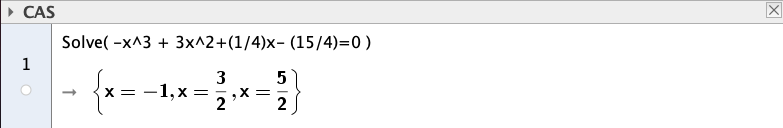
\includegraphics[scale=0.5]{tredjegrad.png}
\end{center}
\caption{Ligningen løst med CAS}
\label{fig:tredjegrad}
\end{figure}
\noindent\textbf{b.}
Vi bemærker, at kun skæringspunkterne $\left(\frac{3}{2},\frac{15}{8}\right)$ og $\left(\frac{5}{2},\frac{21}{8}\right) $ fra \textbf{a.} er i første kvadrant 
Ved at kigge på figuren i opgavebeskrivelsen ses det, at $f(x)\geq g(x)$ for alle $x \in \left[\frac{3}{2},\frac{5}{2}\right]$. 
Siden det er de to grafer, der afgrænser området $M$, så må $M$ være
\[
M=\{(x,y): \frac{3}{2}\leq x \leq \frac{5}{2} \land g(x) \leq y \leq f(x)\}
\] 
$f$ og $g$ er begge kontinuerte funktioner. 
Altså gælder der, at
\begin{equation*}
\begin{split}
  A(M)&=\int_{\frac{3}{2}}^{\frac{5}{2}} \left(f(x)-g(x)\right)  \,dx \\ 
  &=\int_{\frac{3}{2}}^{\frac{5}{2}} \left(-x^3+3x^2+x-3-\frac{3}{4}x-\frac{3}{4}\right)  \,dx \\ 
  &=\int_{\frac{3}{2}}^{\frac{5}{2}} \left(-x^3+3x^2+\frac{1}{4}x-\frac{15}{4}\right)  \,dx \\ 
  &=-\frac{1}{4}\left[x^4\right]_{\frac{3}{2}}^{\frac{5}{2}}+\left[x^3\right]_{\frac{3}{2}}^{\frac{5}{2}}+\frac{1}{8}\left[x^2\right]_{\frac{3}{2}}^{\frac{5}{2}}-\frac{15}{4}\left[x\right]_{\frac{3}{2}}^{\frac{5}{2}}\\ 
  &=\frac{1}{2}
\end{split}
\end{equation*}
Arealet af $M$ er altså $\frac{1}{2}$. \\[1ex]
\textbf{c.}
Da det er graferne for $f$ og $g$, der afgrænser $M$, så må omkredsen af $M$ være summen af kurvelængderne af graferne for $f$ og $g$ i intervallet $x \in \left[\frac{3}{2},\frac{5}{2}\right]$ (som vi betegner $L_f$ og $L_g$).
Bemærk, at siden $g$ er en lineær funktion, så kan $L_g$ regnes med pythagoras. 
$L_f$ regnes med CAS (se \cref{fig:L_f}).
\begin{equation*}
\begin{split}
  O(M)&=L_f+L_g\\ 
  &=\int_{\frac{3}{2}}^{\frac{5}{2}} \sqrt{1+f'(x)^2}  \,dx + \sqrt{\left(\frac{5}{2}-\frac{3}{2}\right) ^2+\left(\frac{21}{8}-\frac{15}{8}\right)^2 } \\
  &=\int_{\frac{3}{2}}^{\frac{5}{2}} \sqrt{1+ \left(-3x+6x+1\right)^2}  \,dx +\frac{5}{4}\\ 
  &\approx 2,017 + \frac{5}{4}\\ 
  &=3,267
\end{split}
\end{equation*}
Omkredsen af $M$ er altså $3,267$. 
\begin{figure}[H]
\begin{center}
  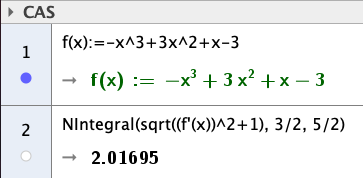
\includegraphics[scale=0.7]{L_f.png}
\end{center}
\caption{$L_f$ beregnet numerisk med CAS}
\label{fig:L_f}
\end{figure}
\begin{question}{}{}
  En funktion $f$ er bestemt ved
$$f(x)=-x^2+4\:.$$
Grafen for $f$ og koordinatsystemets akser afgrænser i første kvadrant en punktmængde $M$, der har et areal.
\begin{itemize}
  \item[a.] Bestem arealet af $M.$
\end{itemize}
Når $0<a<2$, skærer tangenten til grafen for$f$ i punktet $P(a,f(a))$ koordinatsystemets akser i punkterne $Q$ og $R$ (se figuren). Det oplyses, at arealet af trekant $OQR$ er en funktion af $a$, som er givet ved
$$T(a)=\dfrac{(a^2+4)^2}{4a},\:0<a<2.$$
\begin{itemize}
  \item[b.] Bestem den værdi af $a$, der gør arealet af trekant $OQR$ mindst muligt
  \item[c.] Bestem koordinatsættet til hvert af punktern $Q$ og $R$ udtrykt ved $a$, og gør rede for, at arealet af trekant $OQR$ som funktion af $a$ er givet ved $T(a).$
\end{itemize}
\end{question}
\sol \\
\textbf{a.}
Vi løser først ligningen $f(x)= 0$ for at finde det positive nulpunkt.
\begin{equation*}
\begin{split}
  f(x)= 0 &\iff -x^2+4=0\\ 
  &\iff x^2=4\\
  &\iff x=2 \lor x=-2
\end{split}
\end{equation*}
Altså vil det sige, at grafen for $f$ skærer $y$-aksen, når $x=0$, og grafen for $f$ skærer $x$-aksen i første kvadrant når $x=2$. 
Siden $M$ er punktmængden i første kvadrant afgrænset af grafen for $f$ og koordinatsystemets akser, så må arealet være
\begin{equation*}
\begin{split}
  A(M)&=\int_{0}^{2} f(x) \,dx \\
  &=\int_{0}^{2} \left( -x^2+4\right) \,dx \\
  &=-\frac{1}{3}\left[x^3\right]_{0}^{2} + 4 \left[x\right]_{0}^{2}\\
  &=-\frac{8}{3}+8\\ 
  &=\frac{16}{3}
\end{split}
\end{equation*}
Arealet af punktmængden $M$ er altså $\frac{16}{3}$.\\[1ex]
\textbf{b.}
Vi finder først den afledede funktion af $T$ med hensyn til $a$ via produktreglen. 
\begin{equation*}
\begin{split}
  T'(a)&=\dv{a} \left(\frac{\left(a^2+4\right)^2}{4a}\right) \\ 
  &=\dv{a} \left(\left(a^2+4\right)^2\right) \cdot \frac{1}{4a} + \left(a^2+4\right)^2 \cdot \frac{1}{4} \cdot \dv{a} \left(\frac{1}{a}\right) \\
  &=2 \cdot \left(a^2+4\right) \cdot 2a \cdot \frac{1}{4a} + \left(a^2+4\right)^2 \cdot \frac{1}{4} \cdot \left(-\frac{1}{a^2}\right)  \\ 
  &=\left(a^2+4\right) -\frac{\left(a^2+4\right)^2}{4a^2}\\ 
  &=a^2+4-\frac{a^2}{4}-\frac{4}{a^2}-2\\ 
  &=\frac{3}{4}a^2-\frac{4}{a^2}+2
\end{split}
\end{equation*}
Vi sætter denne lig 0 og løser for $a$.
\begin{equation*}
\begin{split}
  T'(a)=0 &\implies \frac{3}{4}a^2-\frac{4}{a^2}+2=0\\ 
  &\iff \frac{3a^4-16+8a^2}{4a^2}=0\\
  &\iff 3a^4+8a^2-16=0
\end{split}
\end{equation*}
Vi laver nu en substitution med $u=a^2$.
\begin{equation*}
\begin{split}
  3a^4+8a^2-16=0 &\iff 3u^2+8u-16=0\\
  &\iff \left(u+4\right) \left(3u-4\right) =0\\ 
  &\iff u=-4 \lor u=\frac{4}{3}\\ 
  &\iff a=\pm \sqrt{-4} \lor a=\pm \sqrt{\frac{4}{3}} 
\end{split}
\end{equation*}
Imidlertid er $Dm(T)=]0;2[$, og vi har da, at 
\[
a=\sqrt{\frac{4}{3}} =\frac{2}{\sqrt{3}}
\] 
Vi ser, at $0<1<\frac{2}{\sqrt{3} }$, og beregner $T'(1)$.
\begin{equation*}
\begin{split}
  T'(1)&=\frac{3}{4}\cdot 1^2-\frac{4}{1^2}+2\\ 
  &=-\frac{5}{4}<0
\end{split}
\end{equation*}
Vi ser også, at $\frac{2}{\sqrt{3} }<\frac{4}{3}<2$, og beregner $T'\left(\frac{4}{3}\right) $.
\begin{equation*}
\begin{split}
  T'\left(\frac{4}{3}\right) &=\frac{3}{4}\cdot \frac{4^2}{3^2}-\frac{4 \cdot 3^2}{4^2}+2\\
  &=\frac{4}{3}-\frac{3^2}{4}+2\\ 
  &=\frac{13}{12}>0
\end{split}
\end{equation*}
Siden $T'(a)$ er kontinuert i intervallet $]0;2[$, samt at $T'(1)<0$ og $T'\left(\frac{4}{3}\right)>0$ er det klart, at $\frac{2}{\sqrt{3} }$ må være et minimumssted. 
Arealet af trekant $OQR$ er altså mindst muligt, når $a=\frac{2}{\sqrt{3} }$. \\[1ex]
\textbf{c.}
Ligningen for tangenten til grafen for $f$ i punktet $P(a,f(a))$ er
\begin{equation*}
\begin{split}
  y&=f'(a) \cdot \left(x-a\right) +f(a)\\
  &=-2a \cdot (x-a) - a^2+4\\
  &=a^2-2ax+4
\end{split}
\end{equation*}
Da punktet $R$ ligger på $y$-aksen, så må $x$-værdien være 0. 
Da gælder da
\begin{equation*}
\begin{split}
  y&=a^2-2a \cdot 0 +4\\
  &=a^2+4
\end{split}
\end{equation*}
Altså har vi $R=(0,\,a^2+4)$.
Siden punktet $Q$ ligger på $x$-aksen, så må dets $y$-værdi være 0.
Da gælder da
\begin{equation*}
\begin{split}
  0=a^2-2ax+4 \iff x=\frac{a^2+4}{2a}
\end{split}
\end{equation*}
Altså må $Q$ udtrykt ved $a$ være $\left(\frac{a^2+4}{2a},\, 0\right)$.
Arealet af trekant $OQR$ må være $\frac{1}{2} \cdot \abs{OQ} \cdot \abs{OR} $. 
\begin{equation*}
\begin{split}
  A&=\frac{1}{2} \cdot \abs{OQ} \cdot \abs{OR}\\
  &=\frac{1}{2} \cdot \frac{a^2+4}{2a} \cdot \left(a^2+4\right) \\
  &=\frac{\left(a^2+4\right)^2}{4a}\\
  &=T(a)
\end{split}
\end{equation*}
Per definition af punkterne $O$ og $Q$ findes de kun, når $0<a<2$, hvilket stemmer overens med funktionens domæne.
Altså har vi vist, hvad vi ville.
\end{document}
